\section{Buffer Class Reference}
\label{classBuffer}\index{Buffer@{Buffer}}
{\tt \#include $<$buffer.h$>$}

Inheritance diagram for Buffer::\begin{figure}[H]
\begin{center}
\leavevmode
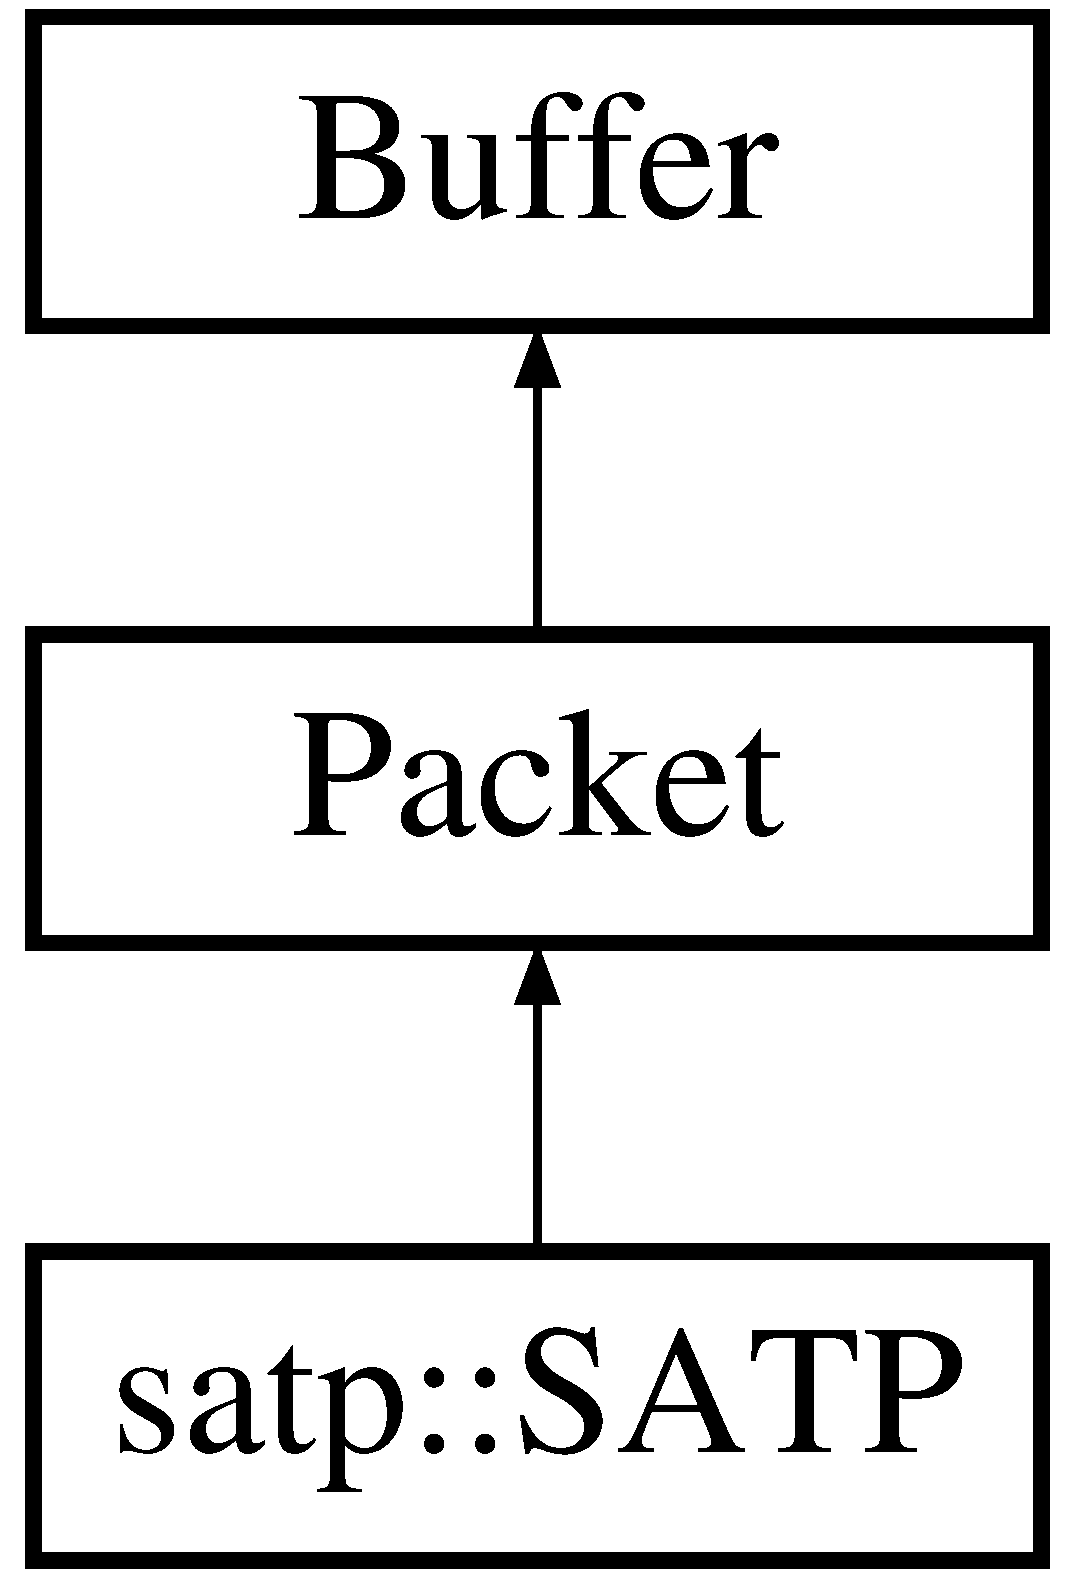
\includegraphics[height=3cm]{classBuffer}
\end{center}
\end{figure}
\subsection*{Public Member Functions}
\begin{CompactItemize}
\item 
{\bf Buffer} ()
\item 
{\bf Buffer} ({\bf u\_\-int32\_\-t} length)
\item 
{\bf Buffer} ({\bf u\_\-int8\_\-t} $\ast$data, {\bf u\_\-int32\_\-t} length)
\item 
virtual {\bf $\sim$Buffer} ()
\item 
{\bf Buffer} (const {\bf Buffer} \&src)
\item 
void {\bf operator=} (const {\bf Buffer} \&src)
\item 
void {\bf operator=} (const {\bf seq\_\-nr\_\-t} \&src)
\item 
void {\bf operator=} (const {\bf sender\_\-id\_\-t} \&src)
\item 
virtual {\bf Buffer} {\bf operator$^\wedge$} (const {\bf Buffer} \&xor\_\-by) const 
\item 
virtual {\bf Buffer} {\bf left\-Byte\-Shift} ({\bf u\_\-int32\_\-t} width) const
\item 
virtual {\bf Buffer} {\bf right\-Byte\-Shift} ({\bf u\_\-int32\_\-t} width) const
\item 
{\bf u\_\-int32\_\-t} {\bf resize\-Front} ({\bf u\_\-int32\_\-t} new\_\-length)
\item 
{\bf u\_\-int32\_\-t} {\bf resize\-Back} ({\bf u\_\-int32\_\-t} new\_\-length)
\item 
{\bf u\_\-int32\_\-t} {\bf get\-Length} () const
\item 
{\bf u\_\-int8\_\-t} $\ast$ {\bf get\-Buf} ()
\item 
{\bf u\_\-int8\_\-t} \& {\bf operator[$\,$]} ({\bf u\_\-int32\_\-t} index)
\item 
{\bf u\_\-int8\_\-t} {\bf operator[$\,$]} ({\bf u\_\-int32\_\-t} index) const
\item 
void {\bf print\-Hex\-Dump} () const
\item 
{\bf operator u\_\-int8\_\-t $\ast$} ()
\end{CompactItemize}
\subsection*{Protected Attributes}
\begin{CompactItemize}
\item 
{\bf u\_\-int8\_\-t} $\ast$ {\bf buf\_\-}
\item 
{\bf u\_\-int32\_\-t} {\bf length\_\-}
\end{CompactItemize}
\subsection*{Friends}
\begin{CompactItemize}
\item 
class {\bf Tun\-Device}
\item 
class {\bf UDPPacket\-Source}
\end{CompactItemize}


\subsection{Constructor \& Destructor Documentation}
\index{Buffer@{Buffer}!Buffer@{Buffer}}
\index{Buffer@{Buffer}!Buffer@{Buffer}}
\subsubsection{\setlength{\rightskip}{0pt plus 5cm}Buffer::Buffer ()}\label{classBuffer_e7ef2cd201190fde551dcb902627112b}


\index{Buffer@{Buffer}!Buffer@{Buffer}}
\index{Buffer@{Buffer}!Buffer@{Buffer}}
\subsubsection{\setlength{\rightskip}{0pt plus 5cm}Buffer::Buffer ({\bf u\_\-int32\_\-t} {\em length})}\label{classBuffer_5c58aa9e491f709011408ee7837d57d0}


\index{Buffer@{Buffer}!Buffer@{Buffer}}
\index{Buffer@{Buffer}!Buffer@{Buffer}}
\subsubsection{\setlength{\rightskip}{0pt plus 5cm}Buffer::Buffer ({\bf u\_\-int8\_\-t} $\ast$ {\em data}, {\bf u\_\-int32\_\-t} {\em length})}\label{classBuffer_5bc2edccfb7c1a33354c895ab25c4816}


\index{Buffer@{Buffer}!~Buffer@{$\sim$Buffer}}
\index{~Buffer@{$\sim$Buffer}!Buffer@{Buffer}}
\subsubsection{\setlength{\rightskip}{0pt plus 5cm}Buffer::$\sim$Buffer ()\hspace{0.3cm}{\tt  [virtual]}}\label{classBuffer_59b8743e4a5f731bdd0c4185c9ef263b}


\index{Buffer@{Buffer}!Buffer@{Buffer}}
\index{Buffer@{Buffer}!Buffer@{Buffer}}
\subsubsection{\setlength{\rightskip}{0pt plus 5cm}Buffer::Buffer (const {\bf Buffer} \& {\em src})}\label{classBuffer_042fe5bc1f8d0c25d5707d6955d1654c}




\subsection{Member Function Documentation}
\index{Buffer@{Buffer}!operator=@{operator=}}
\index{operator=@{operator=}!Buffer@{Buffer}}
\subsubsection{\setlength{\rightskip}{0pt plus 5cm}void Buffer::operator= (const {\bf Buffer} \& {\em src})}\label{classBuffer_14cec0d3bf4f3f1a4a9930a8c53eb43a}


\index{Buffer@{Buffer}!operator=@{operator=}}
\index{operator=@{operator=}!Buffer@{Buffer}}
\subsubsection{\setlength{\rightskip}{0pt plus 5cm}void Buffer::operator= (const {\bf seq\_\-nr\_\-t} \& {\em src})}\label{classBuffer_b62dfbb5605a860aa63771f3b1c29b1e}


\index{Buffer@{Buffer}!operator=@{operator=}}
\index{operator=@{operator=}!Buffer@{Buffer}}
\subsubsection{\setlength{\rightskip}{0pt plus 5cm}void Buffer::operator= (const {\bf sender\_\-id\_\-t} \& {\em src})}\label{classBuffer_b3bda89f495b3895a533155f593ab503}


\index{Buffer@{Buffer}!operator^@{operator$^\wedge$}}
\index{operator^@{operator$^\wedge$}!Buffer@{Buffer}}
\subsubsection{\setlength{\rightskip}{0pt plus 5cm}{\bf Buffer} Buffer::operator$^\wedge$ (const {\bf Buffer} \& {\em xor\_\-by}) const\hspace{0.3cm}{\tt  [virtual]}}\label{classBuffer_d56159a415541fcff34ef8aed1eb7183}


\index{Buffer@{Buffer}!leftByteShift@{leftByteShift}}
\index{leftByteShift@{leftByteShift}!Buffer@{Buffer}}
\subsubsection{\setlength{\rightskip}{0pt plus 5cm}{\bf Buffer} Buffer::left\-Byte\-Shift ({\bf u\_\-int32\_\-t} {\em width}) const\hspace{0.3cm}{\tt  [virtual]}}\label{classBuffer_13200a4925b1b3c08f99e09ccb6854a1}


\index{Buffer@{Buffer}!rightByteShift@{rightByteShift}}
\index{rightByteShift@{rightByteShift}!Buffer@{Buffer}}
\subsubsection{\setlength{\rightskip}{0pt plus 5cm}{\bf Buffer} Buffer::right\-Byte\-Shift ({\bf u\_\-int32\_\-t} {\em width}) const\hspace{0.3cm}{\tt  [virtual]}}\label{classBuffer_298949899f3f78e4a8b3df7fa5ec532d}


\index{Buffer@{Buffer}!resizeFront@{resizeFront}}
\index{resizeFront@{resizeFront}!Buffer@{Buffer}}
\subsubsection{\setlength{\rightskip}{0pt plus 5cm}{\bf u\_\-int32\_\-t} Buffer::resize\-Front ({\bf u\_\-int32\_\-t} {\em new\_\-length})}\label{classBuffer_fe4b10487b4930e0407bdf61857629d6}


\index{Buffer@{Buffer}!resizeBack@{resizeBack}}
\index{resizeBack@{resizeBack}!Buffer@{Buffer}}
\subsubsection{\setlength{\rightskip}{0pt plus 5cm}{\bf u\_\-int32\_\-t} Buffer::resize\-Back ({\bf u\_\-int32\_\-t} {\em new\_\-length})}\label{classBuffer_5698b2d64238f1f38578dc8e9e2b1bc9}


\index{Buffer@{Buffer}!getLength@{getLength}}
\index{getLength@{getLength}!Buffer@{Buffer}}
\subsubsection{\setlength{\rightskip}{0pt plus 5cm}{\bf u\_\-int32\_\-t} Buffer::get\-Length () const}\label{classBuffer_09ced241e4d0a46c52f0f20398076435}


\index{Buffer@{Buffer}!getBuf@{getBuf}}
\index{getBuf@{getBuf}!Buffer@{Buffer}}
\subsubsection{\setlength{\rightskip}{0pt plus 5cm}{\bf u\_\-int8\_\-t} $\ast$ Buffer::get\-Buf ()}\label{classBuffer_7890e20c6c77eb631c39728ea08b35b8}


\index{Buffer@{Buffer}!operator[]@{operator[]}}
\index{operator[]@{operator[]}!Buffer@{Buffer}}
\subsubsection{\setlength{\rightskip}{0pt plus 5cm}{\bf u\_\-int8\_\-t} \& Buffer::operator[$\,$] ({\bf u\_\-int32\_\-t} {\em index})}\label{classBuffer_763882c627db10206f78b090556b00fa}


\index{Buffer@{Buffer}!operator[]@{operator[]}}
\index{operator[]@{operator[]}!Buffer@{Buffer}}
\subsubsection{\setlength{\rightskip}{0pt plus 5cm}{\bf u\_\-int8\_\-t} Buffer::operator[$\,$] ({\bf u\_\-int32\_\-t} {\em index}) const}\label{classBuffer_e5a9559862374ebd9dfcfc1204890497}


\index{Buffer@{Buffer}!printHexDump@{printHexDump}}
\index{printHexDump@{printHexDump}!Buffer@{Buffer}}
\subsubsection{\setlength{\rightskip}{0pt plus 5cm}void Buffer::print\-Hex\-Dump () const}\label{classBuffer_13d927c471a7516b37bc9ad8fc1741ce}


\index{Buffer@{Buffer}!operator u_int8_t *@{operator u\_\-int8\_\-t $\ast$}}
\index{operator u_int8_t *@{operator u\_\-int8\_\-t $\ast$}!Buffer@{Buffer}}
\subsubsection{\setlength{\rightskip}{0pt plus 5cm}Buffer::operator {\bf u\_\-int8\_\-t} $\ast$ ()}\label{classBuffer_dcf367d5f1b7fced7aa61bb919af7943}




\subsection{Friends And Related Function Documentation}
\index{Buffer@{Buffer}!TunDevice@{TunDevice}}
\index{TunDevice@{TunDevice}!Buffer@{Buffer}}
\subsubsection{\setlength{\rightskip}{0pt plus 5cm}friend class {\bf Tun\-Device}\hspace{0.3cm}{\tt  [friend]}}\label{classBuffer_51b494563d277beb4740f86c519f30fb}


\index{Buffer@{Buffer}!UDPPacketSource@{UDPPacketSource}}
\index{UDPPacketSource@{UDPPacketSource}!Buffer@{Buffer}}
\subsubsection{\setlength{\rightskip}{0pt plus 5cm}friend class {\bf UDPPacket\-Source}\hspace{0.3cm}{\tt  [friend]}}\label{classBuffer_940a382a5e3a8622e6689e13dc453481}




\subsection{Member Data Documentation}
\index{Buffer@{Buffer}!buf_@{buf\_\-}}
\index{buf_@{buf\_\-}!Buffer@{Buffer}}
\subsubsection{\setlength{\rightskip}{0pt plus 5cm}{\bf u\_\-int8\_\-t}$\ast$ {\bf Buffer::buf\_\-}\hspace{0.3cm}{\tt  [protected]}}\label{classBuffer_e60240b77a315e6b3c2bf88592d0be48}


\index{Buffer@{Buffer}!length_@{length\_\-}}
\index{length_@{length\_\-}!Buffer@{Buffer}}
\subsubsection{\setlength{\rightskip}{0pt plus 5cm}{\bf u\_\-int32\_\-t} {\bf Buffer::length\_\-}\hspace{0.3cm}{\tt  [protected]}}\label{classBuffer_d3a779d2403b5183427f12554e2f51c3}




The documentation for this class was generated from the following files:\begin{CompactItemize}
\item 
{\bf buffer.h}\item 
{\bf buffer.cpp}\end{CompactItemize}
